\section{Methodology}
\label{sec:Methodology}

\subsection{Preliminary}
Since the method proposed in this paper is based on the Stable Diffusion~\cite{rombach2022high} (SD), we first provide a brief overview of it. SD is a latent diffusion model (LDM) capable of transforming Gaussian noise into high-fidelity images through an iterative denoising process. LDM operates diffusion processes in a latent space, requiring an autoencoder that includes an encoder and decoder. We denote the encoder as $\mathcal{E}(\cdot)$, which encodes an image $I$ into the latent space $z=\mathcal{E}(I)$; similarly, the decoder is denoted as $\mathcal{D}(\cdot)$, used for decoding from the latent space back to the image. Given an input text prompt $y$, the text encoder $c_{\theta}(\cdot)$ of a pre-trained CLIP~\cite{radford2021learning} converts it into a text embedding $c_{\theta}(y)$, which will serve as the input condition for LDM. During training, given a latent noise $z_{t}$ at time step $t$ and condition $c_{\theta}(y)$, the denoising network $\epsilon_{\theta}(\cdot)$ aims to predict noise $\epsilon$. This learning process is facilitated by minimizing the following loss function:
\begin{equation}
\mathcal{L}=\mathbb{E}_{z \sim \mathcal{E}(I), y, \epsilon \sim \mathcal{N}(0,1), t}\left[\left\|\epsilon-\epsilon_\theta\left(z_t, t, c_{\theta}(y)\right)\right\|_2^2\right],\label{eq1}
\end{equation}
The denoising network $\epsilon_{\theta}(\cdot)$ is commonly implemented by U-Net~\cite{ronneberger2015u}. When condition $c_{\theta}(y)$ extracted from the text model is integrated into the denoising network $\epsilon_{\theta}(\cdot)$, the cross-attention layer is needed to achieve cross-modal interaction. The process can be described as follows:
% \begin{equation}
% \begin{aligned}
% \mathbf{Q} & =\mathbf{W}_{Q} \cdot x,\\
% \mathbf{K} & =\mathbf{W}_{K} \cdot c_{\theta}(y),\\
% \mathbf{V} & =\mathbf{W}_{V} \cdot c_{\theta}(y),\label{eq2}
% \end{aligned}
% \end{equation}
\begin{equation}
\mathbf{Q}=\mathbf{W}_{Q} \cdot x, \mathbf{K_c}=\mathbf{W}_{K_c} \cdot c_{\theta}(y), \mathbf{V_c}=\mathbf{W}_{V_c} \cdot c_{\theta}(y),\label{eq2}
\end{equation}
\begin{equation}
\operatorname{Attention}\left(\mathbf{Q}, \mathbf{K_c}, \mathbf{V_c}\right)=\operatorname{softmax}\left(\frac{\mathbf{Q} \mathbf{K_c}^T}{\sqrt{d}}\right)\mathbf{V_c},\label{eq3}
\end{equation}
where $x$ is the spatial feature extracted from latent noise $z$, $\mathbf{W}_{Q}, \mathbf{W}_{K}, \mathbf{W}_{V}$ are learnable projection layers, and $d$ correlates with the number of channels in $x$.

\subsection{The Disentanglement Text Prompts}\label{sec3.2}
This paper aims to further enhance generation quality by integrating aesthetic knowledge across different dimensions. For most fine-tuning approaches~\cite{ruiz2023dreambooth,gal2022image}, the condition is solely derived from the text embedding decoded by the text model from the input text prompt, which encompasses high-level semantic information about the crucial objects and corresponding attributes of an image. In this case, even if there are some aesthetic words in the input text prompt, after several transformer layers, the information can easily \textit{drown} in the process of self-attention with other words, resulting in a minimal cross-modal interaction contribution in U-Net and unsatisfactory performance. On the other hand, the excessive inclusion of aesthetic words, which makes the input prompt overly long, could lead to the inability to generate certain subjects within the prompt.

As illustrated in \cref{Figure 1}, to solve this problem, we initially disentangle the input text prompt of text-to-image synthesis into content and aesthetic input, with aesthetic input $y_{aes}$ being the fine-grained aesthetic labels we introduce, and content input $y$ about the depiction of the main subject and associated attributes in the image. Our starting point comes from the belief that the model can disentangle style (i.e., aesthetics in this case) and content, which is well-documented in~\cite{wu2023uncovering}. 

To enhance the integration of fine-grained aesthetic conditions with the denoising network, we will first introduce the initialization stage of the aesthetic embedding (AesEmb). This phase results in a preprocessed AesEmb that will be consistently utilized throughout both training and inference stages. As shown in \cref{Figure 1}(a), we denote a set of opposing aesthetic labels, where $y_{a}$ denotes a specific aesthetic label (e.g.\ vibrant color, natural lighting, proportional composition, etc.), and $\hat{y}_{a}$ indicates \textit{not having} that label. Notably, we use [identifier] to signify $\hat{y}_{a}$, which is a rare token acting as a unique identifier associated with the aesthetic label (e.g.\ [V], [S])~\cite{ruiz2023dreambooth}. In this context, we employ a rare token to represent $\hat{y}_{a}$ to prevent the semantic prior of the text model from leaking into the negative aesthetic labels. This pair of opposing aesthetic labels $y_p=\{y_{a}, \hat{y}_{a}\}$ is then processed by a frozen CLIP model, yielding a pair of [CLS] tokens, denoted as $t_p=\{t_{cls}, \hat{t}_{cls}\}$.

In practice, more than one set of opposing aesthetic labels is required. Accordingly, we define $N$ sets of aesthetic labels as $\textbf{Y}=\left[y_{p}^{1}, y_{p}^{2}, \ldots, y_{p}^{N}\right]$, where $y_p^i=\{y_{a}^i, \hat{y}_{a}^i\}$ represents the $i$th pair of aesthetic labels. Then we get $N$ sets of [CLS] tokens as $\textbf{T}=\left[t_{p}^{1}, t_{p}^{2}, \ldots, t_{p}^{N}\right]$, where $t_p^i=\{t_{a}^i, \hat{t}_{a}^i\}$ is the $i$th pair of [CLS] tokens generated by the CLIP model. We further concatenate $\textbf{T}$ along the token dimension to obtain our final AesEmb:
\begin{equation}
f_{aes}=\operatorname{concat}\left[t_{p}^{1}, t_{p}^{2}, \ldots, t_{p}^{N}\right] \in \mathbb{R}^{2N \times d},\label{eq5}
\end{equation}
where $f_{aes}$ is the AesEmb and $d$ is the feature dimension. 
It should be emphasized that the initialization of AesEmb requires only a single execution at the start of training and can be cached locally, making the increase in computational cost practically negligible throughout the entire training process.

\begin{figure*}[ht]
	\centerline{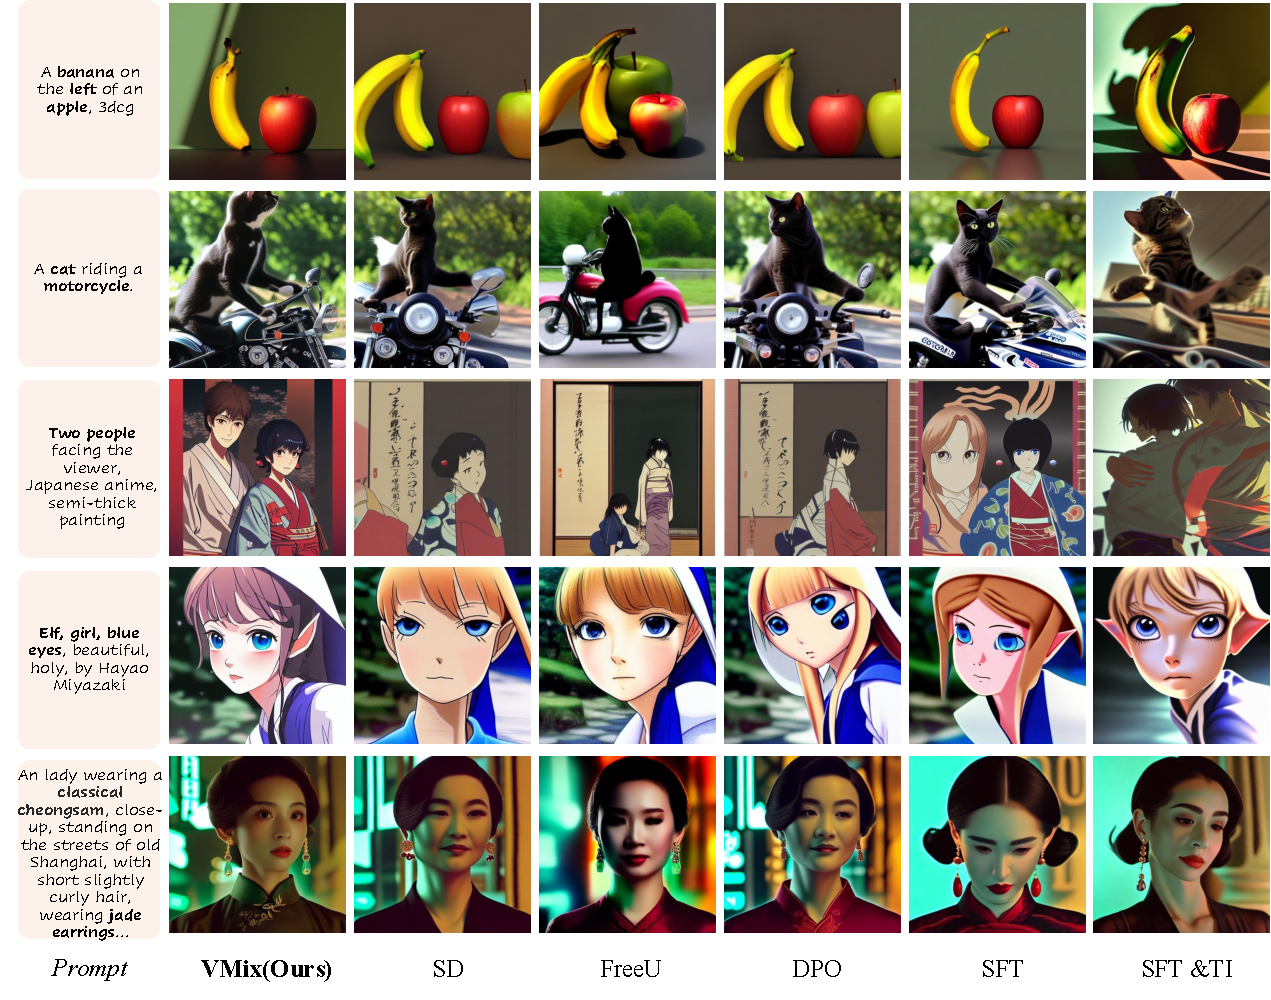
\includegraphics[scale=0.706]{vmix_compare_sd15.pdf}}
	\caption{Qualitative comparison with various state-of-the-art methods. All results are based on Stable Diffusion~\cite{rombach2022high}. Our VMix method outperforms others, significantly enhancing the quality of image generation across various fine-grained aesthetic dimensions.}
	\label{fig4}
\end{figure*}

\begin{figure*}[ht]
	\centerline{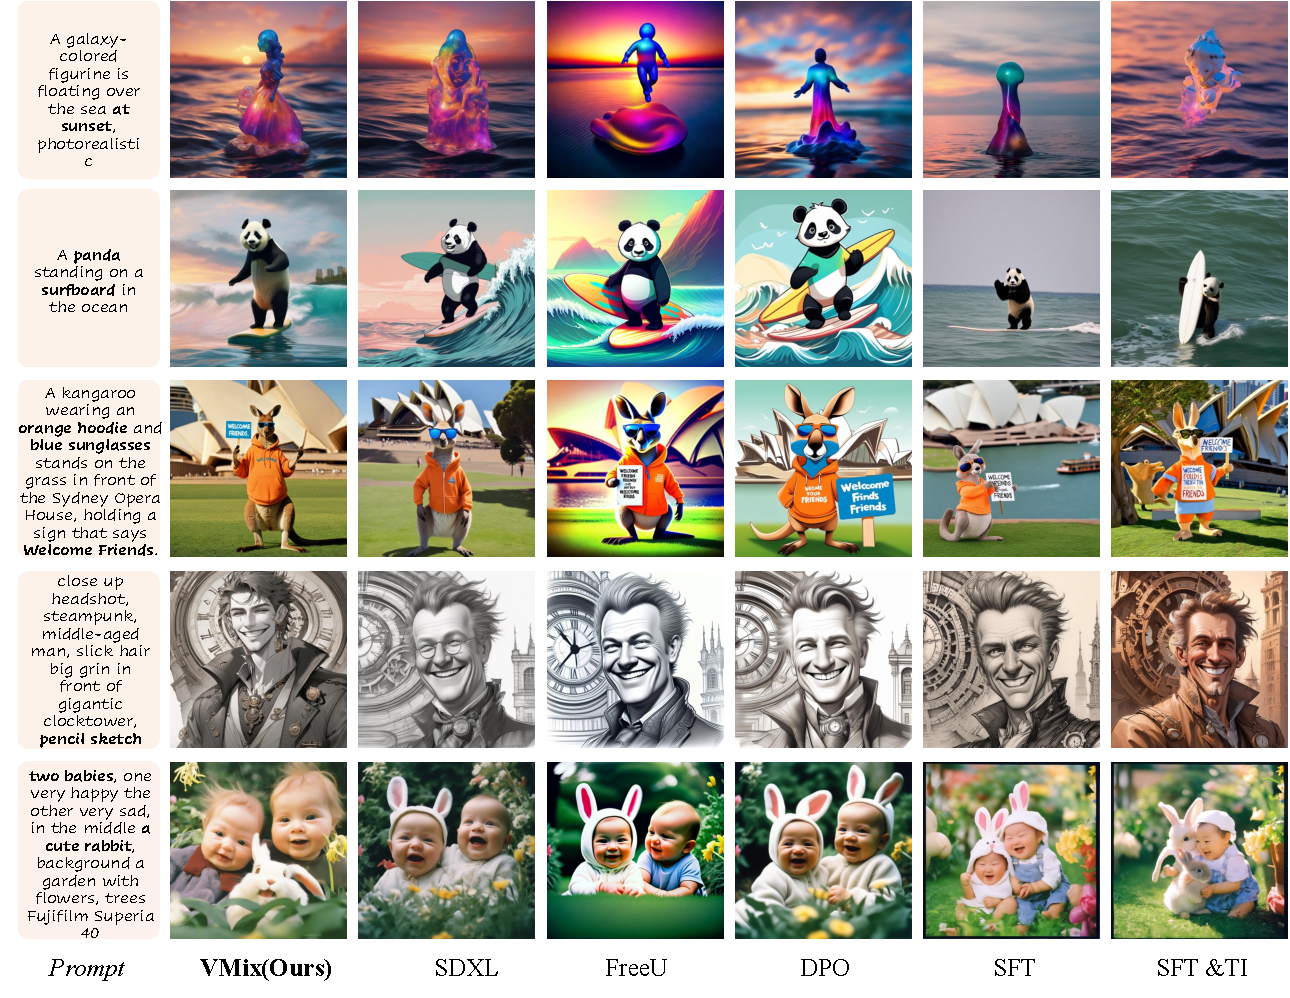
\includegraphics[scale=0.71]{vmix_compare_sdxl2.pdf}}
	\caption{Qualitative comparison with various state-of-the-art methods. All the results of the methods are based on the SDXL~\cite{podell2023sdxl}. Our VMix method outperforms others, significantly enhancing the quality of image generation.}
	\label{fig5}
\end{figure*}
% Our VMix method outperforms others, significantly enhancing the quality of image generation.
\subsection{Cross-Attention Mixing Control}
In the previous section, we disentangle the input text prompt into aesthetic input $y_{aes}$ and content input $y$, and introduce the initialization method for AesEmb. In this section, we will further present an effective and nuanced scheme of condition control that leverages fine-grained aesthetic information to enhance the generative quality of the text-to-image model.

\noindent \textbf{Efficient AesEmb Projection Layer.} As is depicted in \cref{Figure 1}(b), we employ the Stable Diffusion~\cite{rombach2022high} (SD) as our text-to-image model, both $y_{aes}$ and $y$ serving as conditions for the model. Similar to the original SD, the $y$ passes through the text model $c_{\theta}(\cdot)$ of CLIP model~\cite{radford2021learning} and is decoded to obtain the text embedding $f_c$, which can be represented by the following equation:
\begin{equation}
f_c=c_{\theta}(y) \in \mathbb{R}^{C \times d},\label{eq6}
\end{equation}
where $C$ is the token length and $d$ is the feature dimension. Due to the inequity of aesthetic labels in the training dataset, where each image is assigned a variable number of aesthetic labels. We consider two approaches to map aesthetic labels into textual features with the same shape as $f_c$. The first method involves directly processing aesthetic labels through the CLIP model to obtain textual feature $c(y_{aes})$, as indicated by \cref{eq6}. Although this approach is straightforward, it introduces certain issues. Firstly, encoding both $y_{aes}$ and $y$ with the text model incurs additional computational costs. More importantly, although we treat different aesthetic dimensions as independent, the attention layers of the text model may potentially compromise this independence.

Given this, we adopt a more efficient method for condition injection. Initially, based on the aesthetic labels included in the input $y_{aes}$, we index the corresponding [CLS] token from AesEmb $f_{aes} \in \mathbb{R}^{2N \times d}$. For the $i$th aesthetic label, we retrieve $t_{a}^i$ if the image has this attribute, otherwise, we obtain $\hat{t}_a^i$. Thus, we can acquire a feature $f_t \in \mathbb{R}^{N \times d}$ reconstituted from $f_{aes}$. Afterward, we use $\mathcal{F}(\cdot)$ to represent the combination of a linear layer and a Layer Normalization~\cite{ba2016layer}, which serve to upscale the token dimension of $f_t$ from $N$ to $C$. To facilitate a gentler condition injection, we also employ a \textit{zero linear} layer, defined as $\mathcal{Z}(\cdot)$, which is a linear layer with both weight and bias initialized to zeros. The entire projection layer is thus computed as follows:
\begin{equation}
f_a=\mathcal{Z}(\mathcal{F}(f_t)),\label{eq7}
\end{equation}
where $f_a$ is the final textual feature projected from aesthetic labels. 
At the start of training, the weights and biases of the zero-initialized linear layer, which serves as the connecting layer, are set to zero. This initialization ensures that fine-tuning the model does not introduce harmful noise, thereby preserving the capabilities of the original pre-trained model~\cite{zhang2023adding}.

\noindent \textbf{Value-Mixed Cross-Attention.} Directly adding aesthetic textual features to the content textual features may compromise rich semantic features, leading to decreased image-text alignment. Since the attention map within the cross-attention layers dictates the probability distribution over the text tokens for each image patch, determining the principal tokens in the image patch~\cite{chefer2023attend}, we aim to preserve this ability inherent in the pre-trained model. This approach ensures a stable enhancement of aesthetic performance while retaining image-text alignment.

To this end, we introduce our value-mixed cross-attention module after each self-attention module in the diffusion U-Net model. We employ a dual-branch cross-attention module, with one branch for feeding in content features $f_c$ and another for aesthetic features $f_a$. The queries for both branches of the cross-attention module are sourced from the spatial feature $x$ of SD, with the keys originating from the content feature $f_c$. However, the sources for the values are distinct; we enable the model to learn a new value for the aesthetic features independently, thus reducing disruption to the original attention map as aesthetic features are fed into the model. The output of cross-attention corresponding to the content description branch shares the same formula as \cref{eq3}, and can be expressed as $\operatorname{Attention}\left(\mathbf{Q}, \mathbf{K_c}, \mathbf{V_c}\right)$. The output of new cross-attention associated with the aesthetic description branch can be formulated as:
\begin{equation}
\mathbf{Q}=\mathbf{W}_{Q} \cdot x, \mathbf{K_c}=\mathbf{W}_{K_c} \cdot f_c, \mathbf{V_a}=\mathbf{W}_{V_a} \cdot f_a,\label{eq8}
\end{equation}
\begin{equation}
\operatorname{Attention}\left(\mathbf{Q}, \mathbf{K_c}, \mathbf{V_a}\right)=\operatorname{softmax}\left(\frac{\mathbf{Q} \mathbf{K_c}^T}{\sqrt{d}}\right)\mathbf{V_a},\label{eq9}
\end{equation}
The cross-attention modules of these two branches share the same attention map $\mathbf{Q} \mathbf{K_c}^T$. Therefore, we only need to add one parameter $\mathbf{W}_{V_a}$ for each cross-attention layer. Subsequently, we add the outputs from the content and aesthetic cross-attention layers to obtain $\hat{x}$, so the complete process of cross-attention mixing control can be represented as follows:
\begin{equation}
\hat{x}=\operatorname{Attention}\left(\mathbf{Q}, \mathbf{K_c}, \mathbf{V_c}\right)+\lambda\operatorname{Attention}\left(\mathbf{Q}, \mathbf{K_c}, \mathbf{V_a}\right),\label{eq10}
\end{equation}
where $\lambda$ is a hyperparameter and set to $1$ during the training phase, $\hat{x}$ is the new spatial feature and will be fed into the subsequent blocks of SD.

% \noindent \textbf{Training Models with LoRA~\cite{hu2021lora}.} 
\subsection{Training and Inference}\label{sec3.4}
Full-parameter training of models incurs high costs, and while this approach may achieve a higher upper limit of performance, it is inconsistent with our goal of plug-in versatility due to its high degree of customization. For this purpose, during the training phase, we freeze the parameters of the base model, training only the AesEmb Projection Layer and the newly added value in the Value-Mixed Cross-Attention. Additionally, we have incorporated LoRA~\cite{hu2021lora} into some of the model's linear layers and convolutional layers, thereby making the model training process more stable and enhancing the applicability. Upon completion, this segment of the network can be directly extracted to form a plug-and-play module, which can be used to enhancing the aesthetic potential of existing models.
% This module is able to extract fine-grained aesthetic features from the input and can be seamlessly integrated into any latent diffusion model, thereby enhancing the aesthetic potential of existing models.

During inference, in addition to the user's prompt $y$, we also require the aesthetic input $y_{aes}$. Unlike the training phase, where the $y_{aes}$ in the training data contains a varying number of positive aesthetic labels (such as "superior light," "inferior color"). During inference, we default to using all positive aesthetic labels as is shown in \cref{Figure 1}(c). This approach aims to enhance the model's generation quality across all aesthetic dimensions. Although we utilized Lora during the training phase, it is not necessary during inference. We will address this aspect in the experimental section with an ablation study.